\section{Quelques modèles de la croissance des plantes}
\label{ann:modele}

\subsubsection{Informatique et modèles géométriques}

L’arrivée des ordinateurs a révolutionné les méthodes de simulation ainsi que
de modélisation des systèmes et l’étude des plantes en a bien sûr profité.
Les ordinateurs ont fait leur apparition presque en même temps que les
modèles agronomes et botaniques. Ainsi, très vite, ils ont été vus comme un
moyen de simuler la structure géométrique complexe des plantes avec le
développement d’arbres combinatoires, binaires et fractals. 
Mais ces structures purement géométriques et trop rigides ne simulent pas
encore bien le développement complexe des plantes.
Les travaux d’Aristide Lindenmayer aboutissent à une grammaire au formalisme
puissant, grammaire générative basée sur le principe de
réécriture~\cite{LSystem}.

\noindent{
\fbox{
  \parbox{\textwidth}{\paragraph{Qu'est-ce qu'un L-Système?}
Un L-Système est noté :
\[ \{ V,S,\omega ,P \}  \]
Une grammaire formelle qui comprend :
\begin{itemize}
\item Un ensemble alphabet \textbf{V}: Ensemble de variable du L-Système
\item Un ensemble de constantes \textbf{S} : Ensemble de constantes servant notamment lors du dessin géométrique.
\item Un axiome de départ $\mathbf{\omega}$ : État initial.
\item Un ensemble de règles \textbf{P} : Règles de production.
\end{itemize}
Un exemple simple : Algues de Lindenmayer
\[ 
  \left\lbrace
		\begin{array}{cl}
		  V &= \{ A, B\} \\
		  S &= \{ \} \\
		  \omega &= A \\
		  P &= ( A\rightarrow AB)\wedge (B\rightarrow A) \\	
     \end{array}
   \right. 
\]
Avec le résultat sur 6 générations :

\begin{itemize}
  \item[$\bullet$] $n=0$, A
  \item[$\bullet$] $n=1$, AB
  \item[$\bullet$] $n=2$, AB A
  \item[$\bullet$] $n=3$, AB A AB
  \item[$\bullet$] $n=4$, AB A AB AB A
  \item[$\bullet$] $n=5$, AB A AB AB A AB A AB
  \item[$\bullet$] $n=6$, AB A AB AB A AB A AB AB A AB AB A
\end{itemize}

Une suite de symboles générée par L-Système peut être prise en entrée par un
programme informatique qui s’en servira pour générer une structure
géométrique, le plus simple étant d’utiliser un turtle en 2D voire en 3D,
ou encore dans un langage orienté objet avec des pointeurs on peut générer
une chaine cellulaire qui évolue. Les symboles dans $V$ sont les parties des plantes dessinées et les symboles dans $S$ donnent des informations sur la façon dont elles sont dessinées, leur orientation par exemple.
}   
}

Ces modèles de L-système conviennent bien à la simulation des structures des
plantes, elles marchent d’autant mieux combinées à la notion de temps
thermique qui ordonne la dynamique de croissance et permettent d’aboutir 
in fine à une architecture fidèle. On constante cependant
qu'elles n’intègrent pas la notion de
production de biomasse et si elles permettent de prédire une structure
finale aussi fidèle que possible, elles ne permettent pas de prédire le
rythme de production. Les écophysiologistes se sont alors efforcés
d’intégrer des mécanismes de plus en plus fins, avec une simulation locale
et géométrique de la photosynthèse, des échanges entre organes par un
système de transport-résistance avec la notion de force de puits. de organes
puits qui puisent la biomasse produite par les organes sources etc… 
Ces systèmes complexes qui permettent enfin une simulation fine au niveau
individuel ne sont pourtant pas adapté à la simulation et encore moins la modélisation d’un grand ensemble de plantes et ceux pour deux raisons : 
\begin{enumerate}
\item \emph{Le coût en ressources de calcul :} il croît avec le temps de la simulation et le nombre d’individus considérés, encore plus si l’on doit considérer les interactions entre les individus.
\item \emph{La difficulté à paramétrer :} dû au grand nombre de paramètre notamment par rapport aux données que l’on peut raisonnablement récolter.
\end{enumerate}

\subsubsection[Le modèle GreenLab]{Le modèle GreenLab : entre modèle individuel et modèle de production}

\begin{figure}[h]
	\begin{center}
  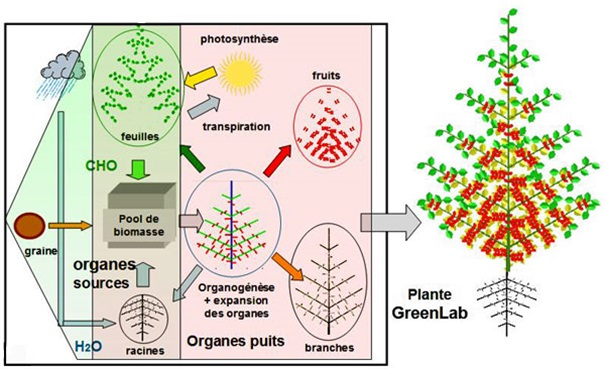
\includegraphics[scale=1]{./img/sGL.jpg}
  \caption{Schéma type d'un modèle GreenLab.}
  \label{fig:schemaGL}
  \end{center}
\end{figure}

Le modèle GreenLab propose une alternative. Il reprend des simplifications utiles du modèle agronome au niveau de la production : la prise en compte de l’architecture individuelle de la plante n’est pas utile au niveau d’un champ, on considère plutôt la distribution des différents types d'organes (densité de feuilles..). Autrement dit, les aspects géométriques peuvent être négligés mais pas la composition quantitative des structures. On fait alors l’hypothèse d’un \emph{pool de biomasse} commun dans lequel les organes vont piocher, et on ne considère que la photosynthèse nette, ie les proportions de glucides qui servent effectivement à la construction de matière sèche des organes. 

Au niveau de l’allocation, cette approche décrit précisément des compartiments d’organes se comportant de façon similaire, ce qui rend l’allocation de biomasse plus facile à modéliser entre organes sources et organes puits et permet de se passer d’une description géométrique ou même topologique exhaustive. Les organes sont générés par cohortes (groupes générés en même temps) de même type grâce à des équations de production des méristèmes selon leur âge physiologique, et des lois de probabilités qui déterminent la croissance, la sénescence et le branching. Et comme tous les organes d’une même cohorte d’organe du même type ont le même état, on peut opérer facilement une factorisation en sous-structures qui rend les calculs plus léger, ainsi le temps de calcul n’est plus proportionnel au nombre d’organe mais seulement à l’âge de la plante. En particulier en multipliant le nombre d’organe de chaque cohorte par la force de puit correspondante et en additionnant le tout on obtient la demande de la plante.

Ensuite l’augmentation $\delta q$ de biomasse de chaque organe est obtenu avec la formule suivante :

\[ \delta q = \phi \cdot Q/D \]

Avec $\phi$ la force de puit, Q la pool de biomasse global et D la demande totale de la plante.

La masse des organes est la somme cumulée de l’augmentation des biomasses, on peut donc obtenir rapidement les dimensions (longueur, diamètre, surface) des organes en utilisant de simples lois géométriques (beaucoup plus simple que celles utilisées lorsque la géométrie est prise en compte dans la production). 

Puis pour que le cycle se répète, la biomasse des compartiments s’obtient  en sommant les cohortes de même organes, en particulier on peut obtenir la masse du feuillage puis la surface foliaire ce qui permettra de déterminer la production de biomasse au prochain cycle. La boucle est bouclée.

Pour résumer, ce modèle est un modèle dynamique de croisance des plantes qui marche par rétroaction entre croissance (production de biomasse) et développement (allocation quantitative et architecture). Le calcul de la production ne prend que peu en compte l’architecture de la plante mais seulement l’équation global de production et les relations sources-puits, ce qui permet des économies de calcul intéressantes et n’empêche pas dans un second temps de générer des structures géométriques fidèles issus d’un modèle de production simplifié mais robuste. Ainsi la plasticité des plantes est très bien représenté par ce modèle et on peut rendre compte de différents phénotypes d’une même espèce dans deux environnement très différents.

\begin{figure}[h]
	\begin{center}
  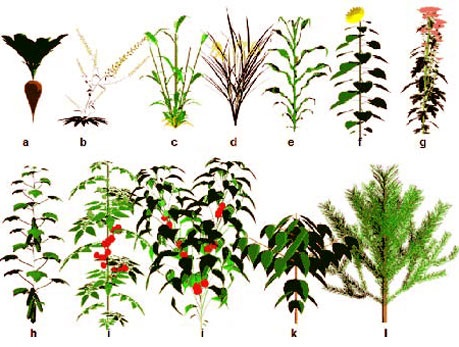
\includegraphics[scale=1]{./img/exempleGL1.jpg}
  \caption{Exemple de plantes générées grâce à GreenLab.}
  \label{fig:exempleGL1}
  \end{center}
\end{figure}

Cela permet notamment la visualisation en images de synthèse très fidèles et complexes de plantes dont la croissance a été modélisé sans prendre en compte le détail géométrique de cette même structure, donc avec un temps de calcul très intéressant. L’augmentation de biomasse de chaque organe a déjà été simplement déterminée grâce aux équations précédentes, dont on déduit également la forme et le volume, de simples règles géométriques positionnent ces organes dans l’architecture selon l’empilement des entre-nœuds autour d’un axe, la phyllotaxie, l’angle de branchement, la courbure des axes, comme on peut le visualiser en Figure~\ref{fig:exempleGL1}.

Comme montré dans la Figure~\ref{fig:exempleP2},
on peut même simuler des paysages entiers grâce à ces méthodes, 
avec le raffinement des paysages fonctionnels qui prennent en compte
raffinement les interactions plantes-environnement, la distribution des
ressources hydriques et des radiations lumineuses entre plantes 
qui sont en compétition.

\begin{figure}[h]
	\begin{center}
	
	
  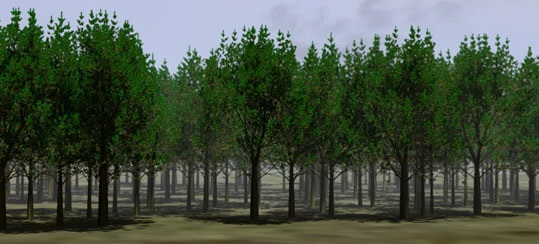
\includegraphics[scale=1.3]{./img/exempleP2.jpg}
  \caption{Paysage fonctionnel généré grâce à GreenLab}
  \label{fig:exempleP2}
  
  \end{center}
\end{figure}